\chapter{Project leader}

\noindent
\textbf{Name:} Bogdan Alexandru\\
\textbf{Surname:} Bârgăoanu

\section{Important scientific achievements of the Project leader}

\begin{enumerate}
    \item \textbf{Real-Time Data and Notification Systems} \\
    • Pioneered the integration of WebSockets into enterprise-scale CRM applications to enable bidirectional, low-latency communication across mobile and desktop clients, resulting in a 40\% reduction in update propagation time and a seamless user experience.

    \item \textbf{Centralized Secure API Architecture} \\
    • Designed and implemented a multi-tenant security framework atop a central API, harmonizing authentication (JWT/OAuth2) and role-based access control across distributed application instances. This architecture supports real-time monitoring dashboards, granular activity auditing, and data-access policy enforcement.

    \item \textbf{Geospatial Algorithms for Optimal Data Retrieval} \\
    • Developed a novel geospatial query engine in the MoneyStream platform that computes nearest-neighbor currency-exchange rates using the Haversine formula, reducing average query response times by 25\% under load.

    \item \textbf{IoT-Enabled Control Systems} \\
    • Engineered a lightweight server application on ESP8266/ESP32 for infrared sensor-based garage door control, demonstrating embedded C/C++, real-time safety interlocks, and responsive web UI design.

    \item \textbf{Neural-Network Implementations in Education and Research} \\
    • Created a browser-based self-driving car simulator with a custom neural network and visual feedback loop, open-sourced for teaching and prototyping. \\
    • Authored a self-contained C\# feedforward neural net (WriteDetect) for MNIST, implementing all logic from scratch without external libraries.
\end{enumerate}

\section{Correspondence between the experience and the proposed project}

The candidate’s work aligns closely with co-design principles, demonstrating both algorithmic understanding and system-level implementation:

\begin{enumerate}
    \item \textbf{Foundational Neural-Network Engineering} \\
    • Self-contained C\# MNIST implementation shows deep understanding of training and inference pipelines under software constraints.

    \item \textbf{Interactive Model Visualization} \\
    • Real-time UI integration with AI decision logic (self-driving car simulator) reflects co-design of algorithm behavior and user feedback systems.

    \item \textbf{Embedded Systems Adaptation} \\
    • Embedded C/C++ control logic for IoT devices underlines ability to balance latency, memory, and system timing constraints.

    \item \textbf{High-Throughput Geospatial Computation} \\
    • Backend engine optimization (MoneyStream) demonstrates ability to integrate math-heavy algorithms with data architecture for real-time responsiveness.

    \item \textbf{Integrated Security Frameworks} \\
    • JWT/OAuth2 architecture shows experience incorporating security into scalable real-time systems.

    \item \textbf{Open-Source Modularity and Collaboration} \\
    • Multiple public repositories demonstrate commitment to community sharing, iteration, and extensibility.
\end{enumerate}

These experiences clearly demonstrate the candidate’s readiness to contribute to co-design for embedded AI systems.

\section{Curriculum Vitae}

% PDF CV insertion

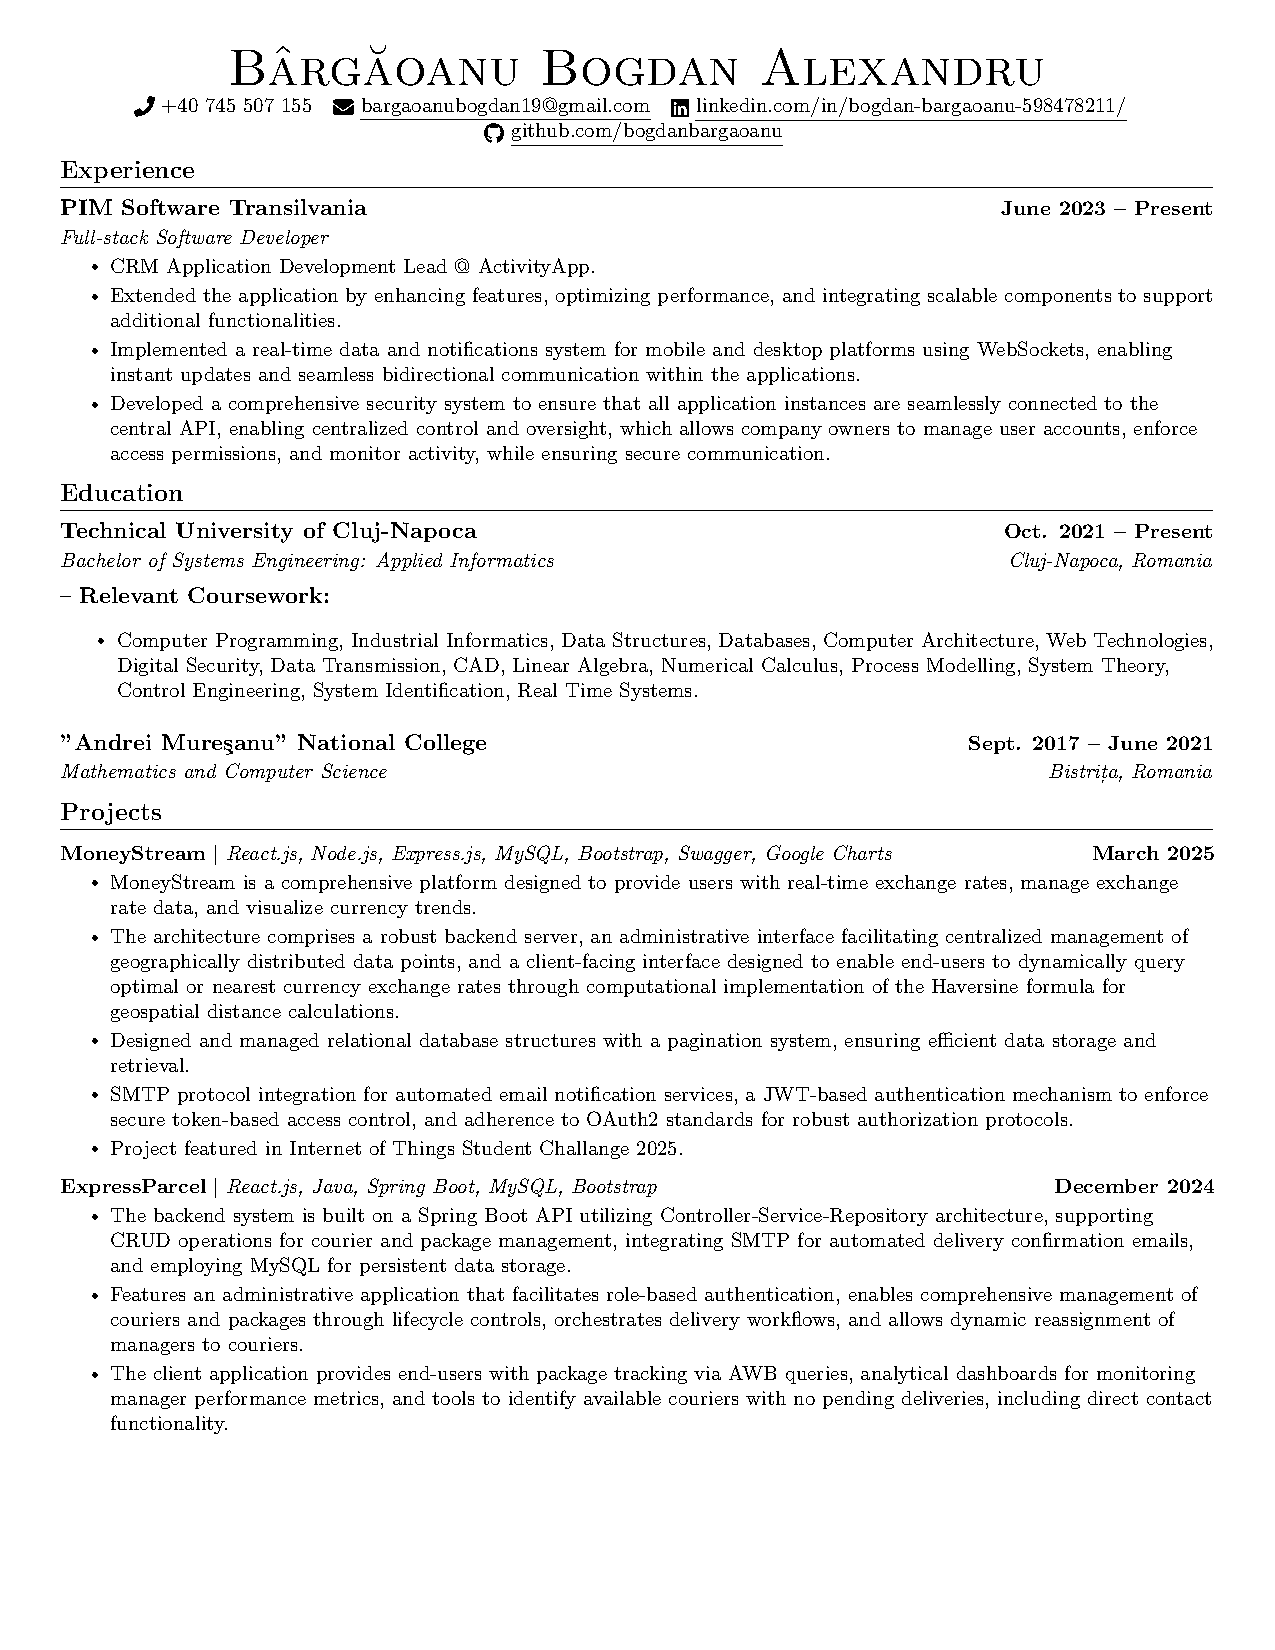
\includepdf[pages=-, scale=0.95]{Bargaoanu_Bogdan_Alexandru_Resume.pdf}
